% Drawing 142/06-18 -- folder 142, batch 06, archive page 117 (PDF page 118).
% Transcription: Au milieu à gauche, une étoile de triangles hachurés autour d'un sommet $1$, avec des sommets $0$, $\infty$ alternés sur le pourtour, chemins pointillés et flèches courbes de rotation ; les triangles $r$ et $\tau_1 r$ sont marqués.
% Kind: star of hatched triangles round a vertex. Method 2 (schematic redraw from the facsimile). Status: partial.
% Notes: Schematic: a star of triangles round a central vertex (1), with vertices 0 and infinity alternating on the outline; some triangles hatched in pencil; dotted paths along the outer edges and curved rotation arrows round the centre; r and tau_1 r marked near the centre. The overinked centre (many short arrows) is reduced to a few curved arrows, and the outline is approximate. The prose in the left margin is not drawn.
% Coordinates: 1 unit = 1 mm = 1/100 of the crop width (bbox in page fractions: [0.21, 0.574, 0.5, 0.748]).
% Redrawn by Claude (claude-opus-5-5), issue #73, 2026-11-07; not checked by a human; not compiled (no TeX in the session).
% Rights: reproduces part of the work -- behind RENDER_TRANSCRIPTS, never published by itself.
\documentclass[tikz,border=3pt]{standalone}
\usepackage{amsmath,amssymb}
\usetikzlibrary{patterns,arrows.meta}
\tikzset{pencil/.style={black!45}, struck/.style={black!35}, mark/.style={circle,draw,inner sep=1.3pt}, pt/.style={circle,fill,inner sep=0.9pt}, opt/.style={circle,draw,fill=white,inner sep=1.1pt}}
\begin{document}
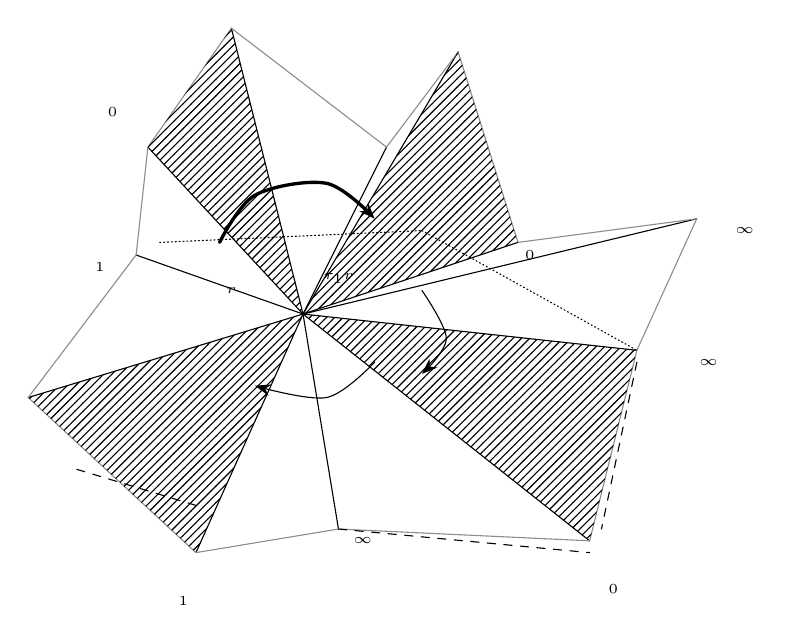
\begin{tikzpicture}[x=1mm,y=1mm,line cap=round,line join=round,font=\scriptsize]
\draw (39.4,-45.4) -- (30.3,-9.1);
\draw (39.4,-45.4) -- (19.7,-24.2);
\draw (39.4,-45.4) -- (18.2,-37.9);
\draw (39.4,-45.4) -- (4.5,-56);
\draw (39.4,-45.4) -- (25.8,-75.7);
\draw (39.4,-45.4) -- (43.9,-72.7);
\draw (39.4,-45.4) -- (75.8,-74.2);
\draw (39.4,-45.4) -- (81.8,-50);
\draw (39.4,-45.4) -- (89.4,-33.3);
\draw (39.4,-45.4) -- (66.7,-36.3);
\draw (39.4,-45.4) -- (59.1,-12.1);
\draw (39.4,-45.4) -- (50,-24.2);
\draw[pencil] (30.3,-9.1) -- (19.7,-24.2) -- (18.2,-37.9) -- (4.5,-56) -- (25.8,-75.7) -- (43.9,-72.7) -- (75.8,-74.2) -- (81.8,-50) -- (89.4,-33.3) -- (66.7,-36.3) -- (59.1,-12.1) -- (50,-24.2) -- cycle;
\fill[pattern=north east lines] (39.4,-45.4) -- (30.3,-9.1) -- (19.7,-24.2) -- cycle;
\fill[pattern=north east lines] (39.4,-45.4) -- (4.5,-56) -- (25.8,-75.7) -- cycle;
\fill[pattern=north east lines] (39.4,-45.4) -- (75.8,-74.2) -- (81.8,-50) -- cycle;
\fill[pattern=north east lines] (39.4,-45.4) -- (66.7,-36.3) -- (59.1,-12.1) -- cycle;
\draw[dashed] (25.8,-69.7) -- (10.6,-65.1);
\draw[dashed] (43.9,-72.7) -- (75.8,-75.7);
\draw[dashed] (81.8,-51.5) -- (77.3,-72.7);
\draw[densely dotted] (54.5,-34.8) -- (81.8,-50);
\draw[densely dotted] (21.2,-36.3) -- (54.5,-34.8);
\draw[-{Stealth[length=2mm]},very thick] plot[smooth, tension=0.55] coordinates {(28.8,-36.3) (33.3,-30.3) (42.4,-28.8) (48.5,-33.3)};
\draw[-{Stealth[length=2mm]}] plot[smooth, tension=0.55] coordinates {(48.5,-51.5) (42.4,-56) (33.3,-54.5)};
\draw[-{Stealth[length=2mm]}] plot[smooth, tension=0.55] coordinates {(54.5,-42.4) (57.6,-48.5) (54.5,-53)};
\node[inner sep=1pt] at (15.2,-19.7) {\tiny $0$};
\node[inner sep=1pt] at (13.6,-39.4) {\tiny $1$};
\node[inner sep=1pt] at (47,-74.2) {\tiny $\infty$};
\node[inner sep=1pt] at (78.8,-80.3) {\tiny $0$};
\node[inner sep=1pt] at (90.9,-51.5) {\tiny $\infty$};
\node[inner sep=1pt] at (68.2,-37.9) {\tiny $0$};
\node[inner sep=1pt] at (95.5,-34.8) {\tiny $\infty$};
\node[inner sep=1pt] at (24.2,-81.8) {\tiny $1$};
\node[inner sep=1pt] at (30.3,-42.4) {\tiny $r$};
\node[inner sep=1pt] at (43.9,-40.9) {\tiny $\tau_1 r$};
\end{tikzpicture}
\end{document}
